\documentclass[final]{scrartcl}

\usepackage[utf8]{inputenc}

\usepackage{fixltx2e}

\usepackage{microtype}
\usepackage{amsmath}
\usepackage{amssymb}
\usepackage{mathtools}
\usepackage{pgfplots}
% \pgfplotsset{compat=1.17}
\pgfplotsset{compat=newest}

\usepackage{amsthm}
\newtheorem*{remark}{Remark}

\newcommand\mytitle{Useful recurrence relations\\
for multidimensional volumes\\
and monomial integrals}
\newcommand\myauthor{Nico Schlömer}

\usepackage[
  pdfencoding=unicode,
  ]{hyperref}
\hypersetup{
  pdfauthor={\myauthor},
  pdftitle={Useful recurrence relations for multidimensional volumes and monomial integrals}
}

% \usepackage[T1]{fontenc}
% \usepackage{newtxtext}
% \usepackage{newtxmath}

% Okay. Don't use biblatex/biber for now. There are breaking changes in every revision,
% and we'd have to stick to the exact version that arxiv.org has, otherwise it's error
% messages like
% ```
% Package biblatex Warning: File 'main.bbl' is wrong format version
% - expected 2.8.
% ```
% \usepackage[sorting=none]{biblatex}
% \bibliography{bib}

\title{\mytitle\footnote{The LaTeX sources of this article are on
\url{https://github.com/nschloe/useful-recurrence-relations}}}
\author{\myauthor}

\begin{document}

\maketitle
\begin{abstract}
  This article gives closed formulas and recurrence expressions for many $n$-dimensional
  volumes and monomial integrals. The recurrence expressions are often much simpler,
  more instructive, and better suited for numerical computation.
\end{abstract}

\subsection*{\textit{n}-dimensional unit cube}
\[
  C_n = \left\{(x_1,\dots,x_n): -1 \le x_i \le 1\right\}
\]

\begin{itemize}
  \item Volume.
    \begin{equation}
      |C_n| = 2^n = \begin{cases}
        1&\text{if $n=0$}\\
        |C_{n-1}| \times 2&\text{otherwise}
      \end{cases}
    \end{equation}
  \item Monomial integration.
  \begin{align}\nonumber
    I_{k_1,\dots,k_n}
    &= \int_{C_n} x_1^{k_1}\cdots x_n^{k_n}\\
      &= \prod_{i=1}^n \frac{1 + (-1)^{k_i}}{k_i+1}
    =\begin{cases}
      0&\text{if any $k_i$ is odd}\\
      |C_n|&\text{if all $k_i=0$}\\
      I_{k_1,\dots,k_{i_0}-2,\dots,k_n} \times \frac{k_{i_0}-1}{k_{i_0}+1}&\text{if $k_{i_0} > 0$}
    \end{cases}
  \end{align}
\end{itemize}

\subsection*{\textit{n}-dimensional unit simplex}
\[
  T_n = \left\{(x_1,\dots,x_n):x_i \geq 0, \sum_{i=1}^n x_i \leq 1\right\}
\]

\begin{itemize}
  \item Volume.
    \begin{equation}
      |T_n| = \frac{1}{n!} = \begin{cases}
        1&\text{if $n=0$}\\
        |T_{n-1}| \times \frac{1}{n}&\text{otherwise}
      \end{cases}
    \end{equation}
  \item Monomial integration.
  % https://math.stackexchange.com/q/207073/36678
  \begin{align}\nonumber
    I_{k_1,\dots,k_n}
    &= \int_{T_n} x_1^{k_1}\cdots x_n^{k_n}\\
    &= \frac{\prod_{i=1}^n\Gamma(k_i)}{\Gamma\left(\sum_{i=1}^n
    k_i\right)}\label{simplex:closed}\\
    &=\begin{cases}
      |T_n|&\text{if all $k_i=0$}\\
      I_{k_1,\dots,k_{i_0}-1,\dots,k_n} \times \frac{k_{i_0}}{n + \sum_{i=1}^n k_i}&\text{if $k_{i_0} > 0$}
    \end{cases}\label{simplex:rec}
  \end{align}
  \begin{remark}
  Note that both numerator and denominator in expression~\eqref{simplex:closed} will
    assume very large values even for polynomials of moderate degree. This can lead to
    difficulties when evaluating the expression on a computer; the registers will
    overflow. A common countermeasure is to use the log-gamma function,
    \[
    \frac{\prod_{i=1}^n\Gamma(k_i)}{\Gamma\left(\sum_{i=1}^n k_i\right)}
    = \exp\left(\sum_{i=1}^n\ln\Gamma(k_i) - \ln\Gamma\left(\sum_{i=1}^n
    k_i\right)\right),
    \]
    but a simpler and arguably more elegant solution is to use the
    recurrence~\eqref{simplex:rec}. This holds true for all such expressions in this
    note.
  \end{remark}

\end{itemize}

\subsection*{\textit{n}-dimensional unit sphere}
\[
  U_n = \left\{(x_1,\dots,x_n): \sum_{i=1}^n x_i^2 = 1\right\}
\]

See also~\cite{tau}.

\begin{itemize}
  \item Volume.
\begin{equation}\label{ndimsphere}
  |U_n|
  = \frac{n \sqrt{\pi}^n}{\Gamma(\frac{n}{2}+1)}
  % = \begin{rcases}\begin{dcases}
  % \frac{n}{(\frac{n}{2})!} \pi^{\frac{n}{2}}&\text{if $n-1$ even}\\
  %   \frac{n2^{n+1}(\frac{n+1}{2})!}{(n+1)!}\pi^{\frac{n-1}{2}}&\text{if $n-1$ odd}
  % \end{dcases}
  % \end{rcases}
  = \begin{cases}
    2&\text{if $n = 1$}\\
    2\pi&\text{if $n = 2$}\\
    |U_{n-2}| \times \frac{2\pi}{n - 2}&\text{otherwise}
  \end{cases}
\end{equation}

  \item Monomial integral~\cite{folland}.
\begin{align}\nonumber
  I_{k_1,\dots,k_n}
  &= \int_{U_n} x_1^{k_1}\cdots x_n^{k_n}\\
  &= \frac{2\prod_{i=1}^n
    \Gamma\left(\frac{k_i+1}{2}\right)}{\Gamma\left(\sum_{i=1}^n\frac{k_i+1}{2}\right)}\label{sphere:closed}\\
  &=\begin{cases}
    0&\text{if any $k_i$ is odd}\\
    |U_n|&\text{if all $k_i=0$}\\
    I_{k_1,\dots,k_{i_0}-2,\dots,k_n} \times \frac{k_{i_0} - 1}{n - 2 + \sum_{i=1}^n k_i}&\text{if $k_{i_0} > 0$}
  \end{cases}
\end{align}
\end{itemize}


\subsection*{\textit{n}-dimensional unit ball}
\[
  S_n = \left\{(x_1,\dots,x_n): \sum_{i=1}^n x_i^2 \le 1\right\}
\]

\begin{itemize}
  \item Volume.

\begin{equation}\label{ndimball}
  |S_n|
  = \frac{\sqrt{\pi}^n}{\Gamma(\frac{n}{2}+1)}
  % = \begin{rcases}
  %   \begin{dcases}
  %     \frac{\pi^{\frac{n}{2}}}{(\frac{n}{2})!}&\text{if $n$ even}\\[1.2ex]
  %     \frac{(\frac{n+1}{2})!2^{n+1}\pi^{\frac{n-1}{2}}}{\left(n+1\right)!}&\text{if $n$ odd}
  % \end{dcases}
  % \end{rcases}
  = \begin{cases}
     1&\text{if $n = 0$}\\
     2&\text{if $n = 1$}\\
     |S_{n-2}| \times \frac{2\pi}{n}&\text{otherwise}
  \end{cases}
\end{equation}

\item Monomial integral~\cite{folland}.
\begin{align}\nonumber
  I_{k_1,\dots,k_n}
  &= \int_{S_n} x_1^{k_1}\cdots x_n^{k_n}\\
  &= \frac{2^{n + p}}{n + p} |S_n|
  =\begin{cases}
    0&\text{if any $k_i$ is odd}\\
    |S_n|&\text{if all $k_i=0$}\\
    I_{k_1,\dots,k_{i_0}-2,\dots,k_n} \times \frac{k_{i_0} - 1}{n - 2 + p}&\text{if $k_{i_0} > 0$}
  \end{cases}
\end{align}
with $p=\sum_{i=1}^n k_i$.
\end{itemize}

\begin{figure}
\centering
% This file was created by tikzplotlib v0.9.2.
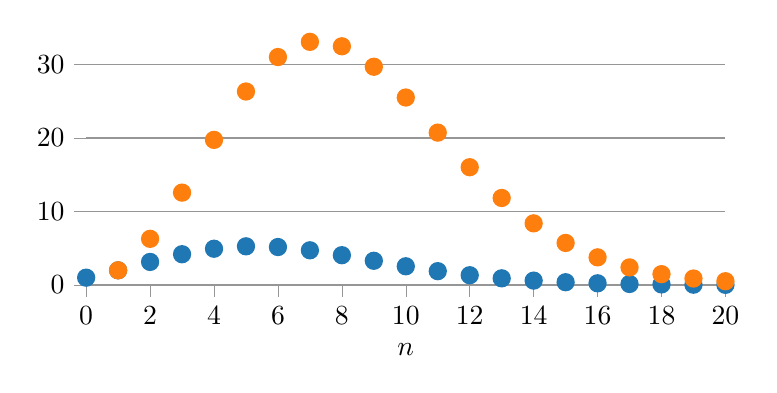
\begin{tikzpicture}

\definecolor{color0}{rgb}{0.12156862745098,0.466666666666667,0.705882352941177}
\definecolor{color1}{rgb}{1,0.498039215686275,0.0549019607843137}

\begin{axis}[
tick align=outside,
tick pos=left,
x grid style={white!58.8235294117647!black},
xlabel={$n$},
xmin=0, xmax=20,
xtick style={color=white!58.8235294117647!black},
y grid style={white!58.8235294117647!black},
ymajorgrids,
ymin=0.0258068913900141, ymax=33.0733617923198,
ytick style={color=white!58.8235294117647!black},
width={0.8\textwidth},
height={0.4\textwidth},
axis line style={draw=none},
ymin=0,
ymax=35
]
\addplot [semithick, color0, mark=*, mark size=3, mark options={solid}, only marks]
table {%
0 1
1 2
2 3.14159265358979
3 4.18879020478639
4 4.93480220054468
5 5.26378901391432
6 5.16771278004997
7 4.7247659703314
8 4.05871212641677
9 3.29850890273871
10 2.55016403987735
11 1.8841038793899
12 1.33526276885459
13 0.910628754783283
14 0.599264529320792
15 0.381443280823304
16 0.235330630358893
17 0.140981106917139
18 0.0821458866111282
19 0.0466216010300885
20 0.0258068913900141
};
\addplot [semithick, color1, mark=*, mark size=3, mark options={solid}, only marks]
table {%
1 2
2 6.28318530717959
3 12.5663706143592
4 19.7392088021787
5 26.3189450695716
6 31.0062766802998
7 33.0733617923198
8 32.4696970113341
9 29.6865801246484
10 25.5016403987734
11 20.7251426732889
12 16.0231532262551
13 11.8381738121827
14 8.38970341049109
15 5.72164921234956
16 3.76529008574229
17 2.39667881759136
18 1.47862595900031
19 0.885810419571682
20 0.516137827800281
};
\draw (axis cs:20.2,-0.641799437700104) node[
  scale=0.7,
  anchor= west,
  text=color0,
  rotate=0.0
]{n-ball};
\draw (axis cs:20.2,1.1837441568904) node[
  scale=0.7,
  anchor= west,
  text=color1,
  rotate=0.0
]{n-sphere};
\end{axis}

\end{tikzpicture}

  \caption{The volumes of the $n$-dimensional ball (and sphere) mysteriously peak at $5$
  (and $7$, respectively). The recurrence relations~\eqref{ndimsphere}
  and~\eqref{ndimball} make it obvious why: The factor $\frac{2\pi}{n}$
  ($\frac{2\pi}{n-2}$) becomes smaller than $1$.}
\end{figure}

\subsection*{\textit{n}-dimensional unit ball with Gegenbauer weight}
  % https://math.stackexchange.com/a/3695653/36678
  $\lambda > -1$. (Compare with~\eqref{ndimball} for $\lambda = 0$.)
  See~\ref{gegenbauer:proof} for a proof.

\begin{itemize}
  \item Volume.
    \begin{align}\nonumber
    |G_n^{\lambda}|
      &= \int_{S^n} \left(1 - \sum_{i=1}^n x_i^2\right)^\lambda\\
      &= \frac{%
        \Gamma(1+\lambda)\sqrt{\pi}^n
      }{%
        \Gamma\left(1+\lambda + \frac{n}{2}\right)
      }
      = \begin{cases}
        1&\text{for $n=0$}\\
        B\left(\lambda+1,\frac{1}{2}\right)&\text{for $n=1$}\\
        |G_{n-2}^{\lambda}|\times \frac{2\pi}{2\lambda + n}&\text{otherwise}
      \end{cases}
  \end{align}

  \item Monomial integration.
  \begin{align}\nonumber
    I_{k_1,\dots,k_n}
      &= \int_{S^n} x_1^{k_1}\cdots x_n^{k_n} \left(1 - \sum_{i=1}^n
      x_i^2\right)^\lambda\\
      &= \frac{%
        \Gamma(1+\lambda)\prod_{i=1}^n \Gamma\left(\frac{k_i+1}{2}\right)
      }{%
        \Gamma\left(1+\lambda + \sum_{i=1}^n \frac{k_i+1}{2}\right)
      }\\
      &= \begin{cases}
        0&\text{if any $k_i$ is odd}\\
        |G_n^{\lambda}|&\text{if all $k_i=0$}\\
        I_{k_1,\dots,k_{i_0}-2,\dots,k_n} \times \frac{k_{i_0}-1}{2\lambda + n + \sum_{i=1}^n k_i}&\text{if $k_{i_0} > 0$}
      \end{cases}
  \end{align}
\end{itemize}


\subsection*{\textit{n}-dimensional unit ball with Chebyshev-1 weight}
% See [Wikipedia](https://en.wikipedia.org/wiki/Chebyshev_polynomials).

Gegenbauer with $\lambda=-\frac{1}{2}$.

\begin{itemize}
  \item Volume.
    \begin{align}\nonumber
    |G_n^{-1/2}|
      &= \int_{S^n} \frac{1}{\sqrt{1 - \sum_{i=1}^n x_i^2}}\\
      &= \frac{%
        \sqrt{\pi}^{n+1}
      }{%
        \Gamma\left(\frac{n+1}{2}\right)
      }
      =\begin{cases}
        1&\text{if $n=0$}\\
        \pi&\text{if $n=1$}\\
        |G_{n-2}^{-1/2}| \times \frac{2\pi}{n-1}&\text{otherwise}
      \end{cases}
    \end{align}

  \item Monomial integration.
    \begin{align}\nonumber
    I_{k_1,\dots,k_n}
      &= \int_{S^n} \frac{x_1^{k_1}\cdots x_n^{k_n}}{\sqrt{1 - \sum_{i=1}^n x_i^2}}\\
      &= \frac{%
        \sqrt{\pi} \prod_{i=1}^n \Gamma\left(\frac{k_i+1}{2}\right)
      }{%
        \Gamma\left(\frac{1}{2} + \sum_{i=1}^n \frac{k_i+1}{2}\right)
      }\\
      &= \begin{cases}
        0&\text{if any $k_i$ is odd}\\
        |G_n^{-1/2}|&\text{if all $k_i=0$}\\
        I_{k_1,\dots,k_{i_0}-2,\dots,k_n} \times \frac{k_{i_0}-1}{n-1 + \sum_{i=1}^n k_i}&\text{if $k_{i_0} > 0$}
      \end{cases}
    \end{align}
\end{itemize}


\subsection*{\textit{n}-dimensional unit ball with Chebyshev-2 weight}
% See [Wikipedia](https://en.wikipedia.org/wiki/Chebyshev_polynomials).
Gegenbauer with $\lambda = +\frac{1}{2}$.

\begin{itemize}
  \item Volume.
    \begin{align}\nonumber
    |G_n^{+1/2}|
      &= \int_{S^n} \sqrt{1 - \sum_{i=1}^n x_i^2}\\
      &= \frac{%
        \sqrt{\pi}^{n+1}
      }{%
        2\Gamma\left(\frac{n+3}{2}\right)
      }
      = \begin{cases}
        1&\text{if $n=0$}\\
        \frac{\pi}{2}&\text{if $n=1$}\\
        |G_{n-2}^{+1/2}| \times \frac{2\pi}{n+1}&\text{otherwise}
      \end{cases}
    \end{align}

  \item Monomial integration.
    \begin{align}\nonumber
    I_{k_1,\dots,k_n}
      &= \int_{S^n} x_1^{k_1}\cdots x_n^{k_n} \sqrt{1 - \sum_{i=1}^n
      x_i^2}\\
      &= \frac{%
        \sqrt{\pi}\prod_{i=1}^n \Gamma\left(\frac{k_i+1}{2}\right)
      }{%
        2\Gamma\left(\frac{3}{2} + \sum_{i=1}^n \frac{k_i+1}{2}\right)
      }\\
      &= \begin{cases}
        0&\text{if any $k_i$ is odd}\\
        |G_n^{+1/2}|&\text{if all $k_i=0$}\\
        I_{k_1,\dots,k_{i_0}-2,\dots,k_n} \times \frac{k_{i_0}-1}{n + 1 + \sum_{i=1}^n k_i}&\text{if $k_{i_0} > 0$}
      \end{cases}
    \end{align}
\end{itemize}


\subsection*{\textit{n}-dimensional generalized Laguerre volume}

$\alpha > -1$. See~\ref{laguerre:proof} for a proof.

\begin{itemize}
  \item Volume.
    \begin{align}\nonumber
  V_n
    &= \int_{\mathbb{R}^n} \left(\sqrt{x_1^2+\cdots+x_n^2}\right)^\alpha \exp\left(-\sqrt{x_1^2+\dots+x_n^2}\right)\\
    &= \frac{2 \sqrt{\pi}^n \Gamma(n+\alpha)}{\Gamma(\frac{n}{2})}
  % = \begin{rcases}\begin{dcases}
  %   \frac{2 \pi^{\frac{n}{2}} (n - 1)!}{(\frac{n}{2} - 1)!} &\text{if $n$ even}\\
  %   \pi^{\frac{n - 1}{2}} 2^n \left(\frac{n - 1}{2}\right)! &\text{if $n$ odd}
  % \end{dcases}
  % \end{rcases}
  = \begin{cases}
    2\Gamma(1+\alpha)&\text{if $n=1$}\\
    2\pi\Gamma(2 + \alpha)&\text{if $n=2$}\\
    V_{n-2} \times \frac{2\pi(n+\alpha-1) (n+\alpha-2)}{n-2}&\text{otherwise}
  \end{cases}
\end{align}

\item Monomial integration.
    \begin{align}\nonumber
  I_{k_1,\dots,k_n}
  &= \int_{\mathbb{R}^n} x_1^{k_1}\cdots x_n^{k_n}
    \left(\sqrt{x_1^2+\dots+x_n^2}\right)^\alpha \exp\left(-\sqrt{x_1^2+\dots+x_n^2}\right)\\
  &= \frac{%
    2 \Gamma\left(\alpha + n + \sum_{i=1}^n k_i\right)
    \left(\prod_{i=1}^n\Gamma\left(\frac{k_i + 1}{2}\right)\right)
  }{%
    \Gamma\left(\sum_{i=1}^n\frac{k_i + 1}{2}\right)
  }\\
  &=\begin{cases}
    0&\text{if any $k_i$ is odd}\\
    V_n&\text{if all $k_i=0$}\\
    I_{k_1,\dots,k_{i_0}-2,\ldots,k_n} \times \frac{%
      (\alpha + n + p - 1) (\alpha + n + p - 2) (k_{i_0} - 1)
    }{%
        n + p - 2
    }&\text{if $k_{i_0} > 0$}
  \end{cases}
\end{align}
with $p=\sum_{k=1}^n k_i$.
\end{itemize}

\subsection*{\textit{n}-dimensional Hermite (physicists')}
\begin{itemize}
  \item Volume.
\begin{align}\nonumber
  V_n
  &= \int_{\mathbb{R}^n} \exp\left(-(x_1^2+\cdots+x_n^2)\right)\\
  &= \sqrt{\pi}^n
%   = \begin{rcases}\begin{dcases}
%      \pi^{\frac{n}{2}}&\text{if $n$ even}\\
%      \sqrt{\pi} \pi^{\frac{n-1}{2}}&\text{if $n$ odd}
%    \end{dcases}
%    \end{rcases}
   = \begin{cases}
     1&\text{if $n=0$}\\
     \sqrt{\pi}&\text{if $n=1$}\\
     V_{n-2} \times \pi&\text{otherwise}
   \end{cases}
\end{align}
%   \item Monomial 1D.
% % See [Wikipedia](https://en.wikipedia.org/wiki/Hermite_polynomials).
% \begin{equation*}
%   \begin{split}
%     I_k
%     &= \int_{-\infty}^\infty x^k \exp(-x^2) dx\\
%     &= \frac{(-1)^k + 1}{2} \times \Gamma\left(\frac{k+1}{2}\right)
%     % = \begin{cases}
%     % \frac{\sqrt{\pi}k!}{2^k (\frac{k}{2})!}&\text{if $k$ even}\\
%     % 0&\text{if $k$ odd}
%     % \end{cases}
%     = \begin{cases}
%       \sqrt{\pi}&\text{if $k = 0$}\\
%       0&\text{if $k = 1$}\\
%       I_{k-2} \times \frac{k-1}{2}&\text{otherwise}
%     \end{cases}
%   \end{split}
% \end{equation*}

  \item Monomial integration.
\begin{align}\nonumber
    I_{k_1,\dots,k_n}
    &= \int_{\mathbb{R}^n} x_1^{k_1}\cdots x_n^{k_n} \exp(-(x_1^2+\cdots+x_n^2))\\
    &= \prod_{i=1}^n \frac{(-1)^{k_i} + 1}{2} \times \Gamma\left(\frac{k_i+1}{2}\right)\\
    &=\begin{cases}
      0&\text{if any $k_i$ is odd}\\
      V_n&\text{if all $k_i=0$}\\
      I_{k_1,\dots,k_{i_0}-2,\dots,k_n} \times \frac{k_{i_0} - 1}{2}&\text{if $k_{i_0} > 0$}
    \end{cases}
\end{align}
\end{itemize}


\subsection*{\textit{n}-dimensional Hermite (probabilists')}
\begin{itemize}
  \item Volume.
    \begin{equation}
      V_n = \frac{1}{\sqrt{2\pi}^n} \int_{\mathbb{R}^n}
      \exp\left(-\frac{1}{2}(x_1^2+\cdots+x_n^2)\right) = 1
    \end{equation}

%   \item Monomial 1D.
% % https://en.wikipedia.org/wiki/Hermite_polynomials
% \[
%   \begin{split}
% I_k
%     &= \frac{1}{\sqrt{2\pi}} \int_{-\infty}^\infty x^k \exp\left(-\frac{1}{2}x^2\right) dx\\
%     &= \frac{(-1)^k + 1}{2} \times \frac{2^{\frac{k+1}{2}}}{\sqrt{2\pi}} \Gamma\left(\frac{k+1}{2}\right)
%     % = \begin{cases}
%     % \frac{k!}{2^{k/2} (\frac{k}{2})!}&\text{if $k$ even}\\
%     % 0&\text{if $k$ odd}
%     % \end{cases}
%     = \begin{cases}
%       1&\text{if $k = 0$}\\
%       0&\text{if $k = 1$}\\
%       I_{k-2} \times (k-1)&\text{otherwise}
%     \end{cases}
%   \end{split}
% \]

  \item Monomial integration.
  \begin{align}\nonumber
    I_{k_1,\dots,k_n}
      &= \frac{1}{\sqrt{2\pi}^n} \int_{\mathbb{R}^n} x_1^{k_1}\cdots x_n^{k_n}
      \exp\left(-\frac{1}{2}(x_1^2+\cdots+x_n^2)\right)\\
    &= \prod_{i=1}^n \frac{(-1)^{k_i} + 1}{2} \times
      \frac{2^{\frac{k_i+1}{2}}}{\sqrt{2\pi}} \Gamma\left(\frac{k_i+1}{2}\right)\\
    &=\begin{cases}
      0&\text{if any $k_i$ is odd}\\
      V_n&\text{if all $k_i=0$}\\
      I_{k_1,\dots,k_{i_0}-2,\dots,k_n} \times (k_{i_0} - 1)&\text{if $k_{i_0} > 0$}
    \end{cases}
  \end{align}
\end{itemize}


\appendix

\section{Some proofs}

\subsection{Gegenbauer}\label{gegenbauer:proof}
\begin{proof}
\[
\begin{split}
\int_{\mathbb{R}^n}  x^{k_1}\cdots x^{k_n} \left(1 - \sum_{i=1}^n x_i^2\right)^\lambda \,dx
&= \int_{S_n}\int_0^1 r^{n-1} r^{\sum{k_i}} (1-r^2)^\lambda x'^{k_1}\cdots x_n'^{k_n} \,dr\,d\sigma(x')\\
&= \int_0^1 r^{n-1} r^{\sum{k_i}} (1-r^2)^\lambda\,dr \times \int_{S_n} x'^{k_1}\cdots x_n'^{k_n} \,d\sigma(x')
\end{split}
\]
with $x_i' = x_i / r$. The one-dimensional integral in $r$ can be evaluated explicitly
  such that, with the spherical integral taken from~\eqref{sphere:closed},
\[
\begin{split}
I_{k_1,\dots,k_n}
&= \frac{\Gamma\left(\frac{n + \sum k_i}{2}\right)\Gamma(1+\lambda)}{2\Gamma\left(\frac{n+\sum k_i}{2} + \lambda + 1\right)}
\times
 \frac{2\prod_{i=1}^n\Gamma\left(\frac{k_i+1}{2}\right)}{\Gamma\left(\sum_{i=1}^n\frac{k_i+1}{2}\right)}\\
  &= \frac{%
  \Gamma(1+\lambda)\prod_{i=1}^n\Gamma\left(\frac{k_i+1}{2}\right)
}{%
\Gamma\left(\sum\frac{k_i+1}{2} + \lambda + 1\right)
}.
\end{split}
\]
\end{proof}

\subsection{Generalized Laguerre}\label{laguerre:proof}
\begin{proof}
\[
\begin{split}
  \int_{\mathbb{R}^n}  x^{k_1}\cdots x^{k_n} r^\alpha \exp(-r) \,dx
  &= \int_{S_n}\int_0^\infty r^{n-1} r^{\sum{k_i}} r^\alpha \exp(-r) x'^{k_1}\cdots x_n'^{k_n} \,dr\,d\sigma(x')\\
  &= \int_0^\infty r^{n-1} r^{\sum{k_i}} r^\alpha \exp(-r)\,dr \times \int_{S_n} x'^{k_1}\cdots x_n'^{k_n} \,d\sigma(x')
\end{split}
\]
with $x_i' = x_i / r$. The one-dimensional integral in $r$ can be evaluated explicitly
  such that, with the spherical integral taken from~\eqref{sphere:closed},
\[
I_{k_1,\dots,k_n}
  = \Gamma\left(\alpha + n + \sum k_i\right) \times
 \frac{2\prod_{i=1}^n\Gamma\left(\frac{k_i+1}{2}\right)}{\Gamma\left(\sum_{i=1}^n\frac{k_i+1}{2}\right)}.
\]
\end{proof}

% \printbibliography{}
\bibliography{bib}{}
\bibliographystyle{plain}

\end{document}
